\documentclass[11pt,letterpaper]{article}

%-----------------------------------------------------------------------------
% Packages
%-----------------------------------------------------------------------------
\usepackage[margin=1in]{geometry}
\usepackage[T1]{fontenc}
\usepackage[utf8]{inputenc}
\usepackage{lmodern}
\usepackage{microtype}
\usepackage{amsmath,amssymb,amsfonts,amsthm}
\usepackage{mathtools}
\usepackage{graphicx}
\usepackage{booktabs}
\usepackage{array}
\usepackage{enumitem}
\usepackage{xcolor}
\usepackage{float}
\usepackage{caption}
\usepackage{subcaption}
\usepackage{hyperref}
\usepackage{authblk}
\usepackage{tikz}
\usetikzlibrary{arrows.meta,positioning,calc,decorations.pathmorphing}

%-----------------------------------------------------------------------------
% Hyperref setup
%-----------------------------------------------------------------------------
\hypersetup{
    colorlinks=true,
    linkcolor=blue!45!black,
    citecolor=blue!45!black,
    urlcolor=blue!45!black
}

%-----------------------------------------------------------------------------
% Theorem environments
%-----------------------------------------------------------------------------
\newtheorem{proposition}{Proposition}
\newtheorem{corollary}{Corollary}
\newtheorem{definition}{Definition}
\newtheorem{remark}{Remark}

%-----------------------------------------------------------------------------
% Commands
%-----------------------------------------------------------------------------
\newcommand{\X}{\ensuremath{\mathcal{X}}}
\newcommand{\Z}{\ensuremath{\mathcal{Z}}}
\newcommand{\ThetaSpace}{\ensuremath{\Theta}}
\newcommand{\EtaSpace}{\ensuremath{\mathcal{E}}}

\newcommand{\Mnominal}{\ensuremath{\mathcal{M}_{\mathrm{N}}}}
\newcommand{\Mhealthy}{\ensuremath{\mathcal{M}_{\mathrm{H}}}}
\newcommand{\Mfault}{\ensuremath{\mathcal{M}_{\mathrm{F}}}}

\newcommand{\Gnuis}{\ensuremath{G_{\mathrm{nuis}}}}
\newcommand{\R}{\ensuremath{\mathbb{R}}}
\newcommand{\quotient}{\ensuremath{\mathcal{X}/G_{\mathrm{nuis}}}}

\newcommand{\residual}{\ensuremath{r}}
\newcommand{\tauadapt}{\ensuremath{\tau_{\mathrm{adapt}}}}
\newcommand{\taumc}{\ensuremath{\tau_{\mathrm{MC}}}}
\newcommand{\mcmu}{\ensuremath{\mu_{\mathrm{MC}}}}
\newcommand{\mcsigma}{\ensuremath{\sigma_{\mathrm{MC}}}}

%-----------------------------------------------------------------------------
% Title
%-----------------------------------------------------------------------------
\title{
\textbf{Anomaly Detection as an Inverse Problem on Quotient Spaces}\\[0.4em]
\large Equivalence Relations and Functional Manifolds as a General Diagnostic Framework\\[0.6em]
\normalsize\itshape Technical Note
}


\author[1]{Eduardo Di Santi}
\affil[1]{Department of Applied Mathematics, University of Colorado Boulder}

\date{June 28, 2026}

\begin{document}
\maketitle

%-----------------------------------------------------------------------------
\begin{abstract}
%-----------------------------------------------------------------------------
This work proposes a quotient-space formulation of diagnostic monitoring in physical systems. The central claim is that anomaly detection is not fundamentally a supervised classification problem in raw observation space, nor does it require identifying the full forward physical model, which may be unknown, nonlinear, high-dimensional, or impractical to learn. Instead, the objective is to recover a representation in which observations that are physically equivalent with respect to the latent state are mapped to the same equivalence class.

The key step is to separate physical-state information from nuisance variability. Measurements are affected by transformations such as amplitude scaling, phase shift, speed variation, sensor offset, installation effects, and additive noise. These transformations modify the observed signal while preserving the underlying physical state. They therefore induce an equivalence relation on the observation space. The resulting quotient space is the natural geometric domain for diagnosis: the inverse problem is no longer posed as explicit recovery of the full generative model, but as recovery of membership in physically meaningful equivalence classes.

Under this formulation, a nominal operating condition is represented not by a single waveform or label, but by a connected functional manifold in the quotient space. Anomaly detection becomes the problem of deciding whether an observation belongs to this nominal quotient manifold. Fault classification, when required, becomes a secondary operation: once an observation is detected outside the nominal manifold, it may be assigned to another quotient-space region or fault manifold. This provides a geometric mechanism for the emergence of functional manifolds: they arise by collapsing nuisance orbits that are irrelevant to the physical state.

After establishing the mathematical object, we introduce one computational approximation. Nominal trajectories are generated by Monte Carlo simulation over nuisance variables, a simple one-dimensional convolutional autoencoder is trained only on the synthetic nominal orbit, and the reconstruction error is used as an inverse-problem residual. An adaptive threshold estimates the local boundary of the nominal manifold for each physical asset. Synthetic validation on four parallel bearing signals provides preliminary evidence that quotient-space recovery is operationally feasible under controlled conditions. The experiments do not prove the mathematical formulation itself; they demonstrate that one computational approximation can recover sufficient quotient geometry to support anomaly detection and subsequent signal classification.
\end{abstract}

%-----------------------------------------------------------------------------
\section{Introduction}
%-----------------------------------------------------------------------------
Diagnostic monitoring in physical systems is often reduced to a pattern recognition problem: given an observation window, assign a semantic label such as nominal, degraded, or faulty. In rotating machinery, this usually becomes a bearing fault classification task, where vibration windows are mapped to labels such as healthy operation, outer-race fault, inner-race fault, or ball fault. This formulation is operationally convenient, and it is well represented in the machinery diagnostics and condition-monitoring literature~\cite{jardine2006,randall2011,zhao2019}. However, it hides a more fundamental structure.

The physical state of a system is not observed directly. Instead, one observes a signal produced by a measurement process that mixes the latent physical state with nuisance factors such as operating speed, amplitude, phase, sensor gain, installation conditions, measurement offsets, and noise. Consequently, two observations can look different in raw signal space while representing the same physical condition. Conversely, two observations can appear superficially similar while belonging to different physical states.

This is the signature of an inverse problem. The observation is not the object of interest; it is the output of a forward process. However, in many industrial settings the full forward model may be unknown, nonlinear, high-dimensional, or impractical to identify. The objective is therefore not necessarily to learn or invert the complete generative model \(F\). The objective is to recover a representation in which physically equivalent observations are identified, while physically meaningful deviations remain detectable. This distinction is related to, but not identical with, classical anomaly and novelty detection formulations~\cite{chandola2009,scholkopf1999,bishop1994}, and to the broader theory of ill-posed inverse problems~\cite{hadamard,tikhonov}.

The central claim of this work is the following:

\begin{quote}
\emph{Diagnostic monitoring can be formulated as inverse recovery over a quotient space induced by nuisance transformations of the observation process.}
\end{quote}

The quotient space appears because nuisance transformations modify the observed signal without changing the underlying physical state. These transformations induce an equivalence relation on the observation space. The diagnostic task can therefore be reformulated as recovery of membership in physically meaningful equivalence classes, rather than direct classification in raw observation space or explicit reconstruction of the full forward physical model. The emphasis on invariance, transformations, and geometry is consistent with the broader geometric learning perspective~\cite{bronstein2021}.

Under this view, a nominal operating condition is not represented by a single waveform or by a predefined label. It is represented by a connected functional manifold in quotient space. Anomaly detection is then a membership test: an observation is nominal if it belongs to the nominal quotient manifold and anomalous if it does not. Classification, when required, becomes a secondary operation: once an observation is detected outside the nominal manifold, it may be assigned to another quotient-space region or fault manifold.

The quotient space is not introduced because an autoencoder is used. The autoencoder is introduced because the diagnostic problem naturally lives on a quotient space. This distinction is essential. The mathematical formulation should remain valid if the computational operator is replaced by another representation learner, such as a contrastive encoder, a predictive latent model, a diffusion-based score model, or a physics-informed residual operator.

This work separates three layers that are often conflated:

\begin{enumerate}[label=(\roman*)]
\item the physical observation model;
\item the quotient-space inverse problem induced by nuisance equivalence;
\item one practical computational approximation.
\end{enumerate}

The first two layers define the scientific contribution. The third layer demonstrates that the formulation can be approximated in a concrete setting. In this work, the concrete setting is a synthetic bearing fault detection experiment, used not as the center of the theory but as a controlled validation of the proposed quotient-space inverse recovery framework.

%-----------------------------------------------------------------------------
\section{Observation Model}
%-----------------------------------------------------------------------------

Let \(\X \subset \R^n\) denote the space of fixed-length observation windows. In the experimental section these observations are vibration windows, but the formulation does not depend on this particular sensing modality.

Let \(\theta \in \ThetaSpace\) denote the latent physical state of the system. In a bearing application, examples of \(\theta\) include nominal operation, outer-race degradation, inner-race degradation, ball damage, or transitional states not yet assigned a semantic label.

Let \(\eta \in \EtaSpace\) denote nuisance variables that modify the observed signal without changing the underlying physical state. Typical nuisance variables include:

\begin{itemize}
    \item amplitude scaling due to gain or load variation;
    \item phase shift due to sampling alignment;
    \item speed perturbation;
    \item DC offset or baseline drift;
    \item sensor placement effects;
    \item additive measurement noise.
\end{itemize}

The observation process is written as
\begin{equation}
    x = F(\theta,\eta), \qquad x \in \X.
    \label{eq:forward_model}
\end{equation}

The diagnostic objective is not to identify \(\eta\). Nor is it necessarily to reconstruct the full forward model \(F\). The diagnostic objective is to recover information about \(\theta\) from \(x\), while remaining invariant to nuisance degrees of freedom. This produces the inverse problem
\begin{equation}
    x \longmapsto \theta,
    \label{eq:inverse_problem}
\end{equation}
or, more precisely, recovery of the physical state modulo nuisance transformations of the observation process.

%-----------------------------------------------------------------------------
\section{Diagnostic Monitoring as Inverse Recovery}
%-----------------------------------------------------------------------------

Equation~\eqref{eq:forward_model} describes a forward observation map.
The inverse diagnostic problem is ill-posed in the classical sense:
multiple nuisance configurations may produce different observations corresponding to the same latent physical state.
The goal is therefore not to invert \(F\) exactly, nor to identify all nuisance variables explicitly.
Instead, the goal is to construct a diagnostic representation
\begin{equation}
    \Phi: \X \rightarrow \Z
    \label{eq:representation}
\end{equation}
such that \(\Phi(x)\) preserves information about the latent physical state while suppressing nuisance variability.

A direct classifier attempts to approximate the map
\[
x \mapsto y,
\]
where \(y\) is a semantic or operational label.
However, the label is not the primitive object.
The primitive object is the latent physical state \(\theta\), and semantic labels are assigned only after a stable diagnostic structure is recovered.

This motivates a two-step view of diagnostic monitoring:

\begin{enumerate}[label=(\alph*)]
    \item recover the geometric structure associated with latent-state equivalence classes;
    \item assign operational semantics to the recovered structures.
\end{enumerate}

In this view, classification is downstream of inverse recovery.
Anomaly detection is not the prediction of a predefined class label.
It is the decision that an observation does not belong to the recovered nominal structure.
If additional non-nominal structures are recovered, subsequent classification may be performed by assigning the observation to another quotient-space region or fault manifold.

The experimental bearing case studied later in this work should therefore be read as one concrete instantiation of this general formulation.
The theory concerns diagnostic monitoring under nuisance transformations; the bearing simulator provides a controlled physical example in which the proposed quotient-space recovery can be evaluated.

%-----------------------------------------------------------------------------
\section{Quotient-Space Formulation}
%-----------------------------------------------------------------------------

The key mathematical object is the equivalence relation induced by nuisance transformations.
Let \(\Gnuis\) denote a group, or approximate transformation family, acting on \(\X\).
For \(g \in \Gnuis\), the transformed observation \(g \cdot x\) represents a change in the measured signal that does not alter the underlying latent physical state.

\begin{definition}[Nuisance equivalence]
Two observations \(x_1,x_2 \in \X\) are nuisance-equivalent, written \(x_1 \sim x_2\), if there exists \(g \in \Gnuis\) such that
\begin{equation}
x_2 = g \cdot x_1,
\label{eq:equivalence}
\end{equation}
and both observations correspond to the same latent physical state \(\theta\).
\end{definition}

The orbit of an observation \(x\) under nuisance transformations is
\begin{equation}
[x] = \{g \cdot x : g \in \Gnuis\}.
\label{eq:orbit}
\end{equation}

The quotient space is the set of such equivalence classes:
\begin{equation}
\quotient = \{[x] : x \in \X\}.
\label{eq:quotient}
\end{equation}

\begin{proposition}[Geometric formulation of diagnostic monitoring]
\label{prop:quotient_diagnosis}
Assume that the nuisance transformations preserve the latent physical state.
That is, for observations generated by \(x=F(\theta,\eta)\), the action of \(g \in \Gnuis\) modifies nuisance degrees of freedom but not \(\theta\).
Then inverse recovery of the latent physical state depends only on the equivalence class \([x]\), not on the particular representative \(x\).
Consequently, the natural domain of diagnostic monitoring is the quotient space \(\X/\Gnuis\), rather than the raw observation space \(\X\).
\end{proposition}

\begin{proof}
Let \(x_1,x_2 \in \X\) satisfy \(x_2=g\cdot x_1\) for some \(g\in\Gnuis\).
By assumption, \(g\) changes only nuisance variables and preserves the latent physical state.
Thus both observations correspond to the same \(\theta\).
Any diagnostic map that recovers information about \(\theta\) must therefore assign the same physical-state information to \(x_1\) and \(x_2\).
Hence the diagnostic map is constant on nuisance orbits and factors through the quotient projection
\[
\pi:\X \rightarrow \X/\Gnuis.
\]
Therefore diagnostic monitoring is naturally posed on the quotient space.
\end{proof}

\begin{corollary}[Equivalence-class diagnosis]
If two observations lie in the same nuisance orbit, no physically meaningful diagnostic decision should distinguish them on the basis of nuisance variation alone.
Consequently, nominal observations should be identified as elements of a nominal equivalence class, or a connected region of such classes, in the quotient space.
\end{corollary}

\begin{definition}[Nominal quotient manifold]
The nominal quotient manifold \(\Mnominal\) is the connected subset of \(\X/\Gnuis\) generated by observations sharing the nominal latent physical state:
\begin{equation}
\Mnominal
=
\{[x] \in \X/\Gnuis : x = F(\theta_{\mathrm{N}},\eta), \ \eta \in \EtaSpace\}.
\label{eq:nominal_manifold}
\end{equation}
\end{definition}

Under this definition, anomaly detection becomes a membership problem:
\begin{equation}
[x] \in \Mnominal
\quad \text{or} \quad
[x] \notin \Mnominal.
\label{eq:membership}
\end{equation}

This is the point at which anomaly detection enters the formulation.
An anomaly is not primarily a label.
It is a failure of membership in the nominal quotient manifold.
Classification, when required, is a subsequent step that assigns non-nominal observations to other quotient-space regions or fault manifolds.

%-----------------------------------------------------------------------------
\section{Functional Manifolds as Quotient Geometry}
%-----------------------------------------------------------------------------

The quotient-space formulation provides a geometric mechanism through which functional manifolds emerge.
A functional manifold is not postulated as an arbitrary structure discovered by an algorithm.
It arises because nuisance transformations generate orbits in observation space, and the quotient projection collapses each orbit into a single equivalence class.

Thus, the observed manifold structure has two sources:

\begin{enumerate}[label=(\roman*)]
    \item physical continuity of the underlying system;
    \item identification of observations that differ only by nuisance transformations.
\end{enumerate}

In raw signal space, nominal operation may appear as a broad, noisy cloud.
In quotient space, the nuisance directions are collapsed.
The remaining geometry is closer to the latent physical-state structure.
This is why learning a representation that is invariant to nuisance transformations can reveal compact functional manifolds.

This mechanism is illustrated conceptually in Figure~\ref{fig:quotient_manifold_concept}.
The quotient projection does not create physical structure \textit{ex nihilo}; it removes directions of variability that are irrelevant to the latent state.
What remains is a lower-complexity geometry in which nominal and non-nominal regimes can be represented as functional manifolds.

\begin{figure}[H]
\centering
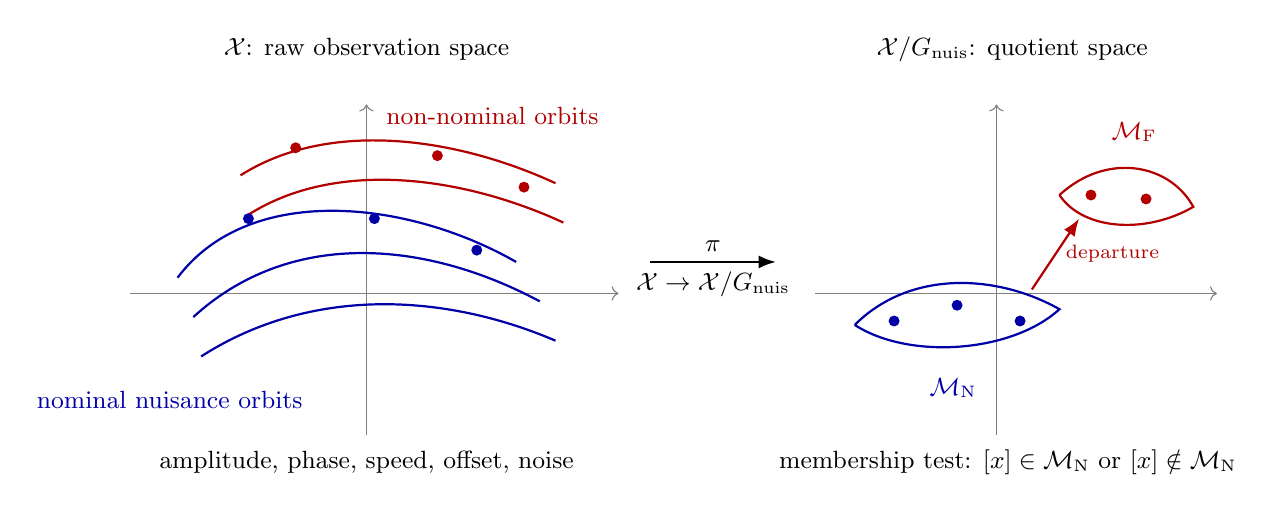
\begin{tikzpicture}[
    scale=1.0,
    every node/.style={font=\small},
    orbit/.style={thick},
    point/.style={circle, fill, inner sep=1.4pt},
    arrow/.style={-{Latex[length=2.2mm]}, thick},
    manifold/.style={thick},
    dashedbox/.style={draw, rounded corners, dashed, inner sep=4pt}
]

% Left panel: raw observation space
\node at (0,3.1) {\(\mathcal X\): raw observation space};

\draw[->, gray] (-3,0) -- (3.2,0);
\draw[->, gray] (0,-1.8) -- (0,2.4);

\draw[orbit, blue!65!black] (-2.4,0.2) .. controls (-1.5,1.4) and (0.5,1.2) .. (1.9,0.4);
\draw[orbit, blue!65!black] (-2.2,-0.3) .. controls (-1.0,0.8) and (0.7,0.7) .. (2.2,-0.1);
\draw[orbit, blue!65!black] (-2.1,-0.8) .. controls (-0.7,0.1) and (1.0,0.0) .. (2.4,-0.6);

\draw[orbit, red!70!black] (-1.6,1.5) .. controls (-0.5,2.2) and (1.1,2.0) .. (2.4,1.4);
\draw[orbit, red!70!black] (-1.5,1.0) .. controls (-0.4,1.7) and (1.2,1.5) .. (2.5,0.9);

\node[point, blue!65!black] at (-1.5,0.95) {};
\node[point, blue!65!black] at (0.1,0.95) {};
\node[point, blue!65!black] at (1.4,0.55) {};

\node[point, red!70!black] at (-0.9,1.85) {};
\node[point, red!70!black] at (0.9,1.75) {};
\node[point, red!70!black] at (2.0,1.35) {};

\node[blue!65!black] at (-2.5,-1.35) {nominal nuisance orbits};
\node[red!70!black] at (1.6,2.25) {non-nominal orbits};

\node at (0,-2.15) {
\(\text{amplitude, phase, speed, offset, noise}\)
};

% Quotient projection arrow
\draw[arrow] (3.6,0.4) -- (5.2,0.4)
node[midway, above] {\(\pi\)}
node[midway, below] {\(\mathcal X \to \mathcal X/G_{\mathrm{nuis}}\)};

% Right panel: quotient space
\node at (8.2,3.1) {\(\mathcal X/G_{\mathrm{nuis}}\): quotient space};

\draw[->, gray] (5.7,0) -- (10.8,0);
\draw[->, gray] (8.0,-1.8) -- (8.0,2.4);

\draw[manifold, blue!65!black] 
    (6.2,-0.4) .. controls (6.9,0.3) and (8.0,0.25) .. (8.8,-0.2)
    .. controls (8.2,-0.75) and (6.9,-0.85) .. (6.2,-0.4);

\node[blue!65!black] at (7.45,-1.2) {\(\mathcal M_{\mathrm{N}}\)};

\draw[manifold, red!70!black] 
    (8.8,1.25) .. controls (9.4,1.8) and (10.2,1.65) .. (10.5,1.1)
    .. controls (9.9,0.75) and (9.1,0.8) .. (8.8,1.25);

\node[red!70!black] at (9.75,2.05) {\(\mathcal M_{\mathrm{F}}\)};

\node[point, blue!65!black] at (6.7,-0.35) {};
\node[point, blue!65!black] at (7.5,-0.15) {};
\node[point, blue!65!black] at (8.3,-0.35) {};

\node[point, red!70!black] at (9.2,1.25) {};
\node[point, red!70!black] at (9.9,1.2) {};

\draw[arrow, red!70!black] (8.45,0.05) -- (9.05,0.95)
node[midway, right] {\scriptsize departure};

\node[align=center] at (8.2,-2.15) {
membership test: \([x] \in \mathcal M_{\mathrm{N}}\) or \([x] \notin \mathcal M_{\mathrm{N}}\)
};

\end{tikzpicture}
\caption{
Conceptual illustration of functional manifolds as quotient geometry.
In raw observation space, nuisance transformations generate extended orbits of observations that preserve the same latent physical state.
The quotient projection \(\pi\) collapses these orbits into equivalence classes, revealing compact nominal and non-nominal functional manifolds.
}
\label{fig:quotient_manifold_concept}
\end{figure}

This also clarifies the relation between anomaly detection and classification.
A classifier learns a partition of labeled observations.
A quotient-space diagnostic operator learns a representation in which physically equivalent observations are identified.
Operational labels may then be attached to the recovered structures, but the structures themselves precede the labels.

%-----------------------------------------------------------------------------
\section{One Computational Approximation}
%-----------------------------------------------------------------------------

The previous sections establish the mathematical object.
We now introduce one computational approximation.

The approximation has four components:

\begin{enumerate}[label=(\arabic*)]
    \item Monte Carlo generation of nominal trajectories over nuisance variables;
    \item self-supervised representation learning on nominal trajectories only;
    \item reconstruction error as an inverse-problem residual;
    \item per-asset adaptive threshold estimation.
\end{enumerate}

This section should be interpreted as one realization of the quotient-space formulation, not as the formulation itself.
The same mathematical framework could be implemented with alternative representation operators, residual functions, or domain simulators.

%------------------------------------------------------------
\subsection{Computational Strategy}
%------------------------------------------------------------

Let \(\theta_{\mathrm{N}}\) denote a nominal latent physical state.
The computational objective is to approximate the nominal quotient manifold \(\Mnominal\) without learning the full forward model \(F\).
Instead of identifying all physical parameters and nuisance variables explicitly, we generate nominal observations under nuisance variability and train a representation operator that is stable on this nominal orbit.

Synthetic nominal samples are generated as
\begin{equation}
x_i = F(\theta_{\mathrm{N}},\eta_i),
\qquad i=1,\ldots,N,
\label{eq:nominal_mc_samples}
\end{equation}
where each \(\eta_i \in \EtaSpace\) represents a nuisance configuration.
These samples approximate the orbit of the nominal state under nuisance transformations.

The purpose of Monte Carlo generation is not to model every possible non-nominal condition.
The purpose is to sample the nominal nuisance orbit densely enough that a representation learner can approximate the quotient geometry of nominal operation.
Non-nominal regimes are then detected by their failure to belong to the recovered nominal structure.

%------------------------------------------------------------
\subsection{Controlled Bearing Instantiation}
%------------------------------------------------------------

The controlled validation uses a synthetic bearing signal emulator designed to expose the geometric structure of the proposed formulation rather than to reproduce a specific industrial asset.
The emulator should not be interpreted as a high-fidelity digital twin of a particular bearing assembly.
Its purpose is to generate regimes with known latent structure, controlled nuisance variability, and controlled non-nominal departures.
This makes it suitable for testing whether the proposed quotient-space approximation can recover membership structure under known ground-truth conditions.

In this instantiation, the generic observation \(x \in \X\) is a vibration window.
Each window has length \(n=1200\), corresponding to \(0.1\) seconds sampled at \(f_s=12{,}000\) Hz.
The nominal shaft frequency is \(30\) Hz.

The nominal bearing signal is generated as a finite harmonic expansion of the shaft frequency:
\[
x_{\mathrm{N}}(t)
=
\sum_{k=1}^{5}
a \rho^{k-1}
\sin(2\pi k f_0 s\,t + \phi/k),
\]
where \(a\) is an amplitude factor, \(\rho=0.55\) is the harmonic decay, \(f_0=30\) Hz is the nominal shaft frequency, \(s\) is a speed-scaling factor, and \(\phi\) is a phase perturbation.

The nuisance variables are sampled by Monte Carlo simulation:
\[
a \sim U(0.85,1.15), \qquad
\phi \sim U(-0.3,0.3), \qquad
s \sim U(0.95,1.05),
\]
together with additive offset, additive noise, and a small local dropout perturbation.
These variables modify the observed waveform without changing the intended physical regime.
They therefore instantiate the nuisance orbit discussed in the quotient-space formulation.

Non-nominal regimes are generated by adding impulsive components to the nominal base signal.
The outer-race fault uses an impulse train near \(108s\) Hz, the inner-race fault uses an impulse train near \(162s\) Hz, and the ball-fault regime uses an impulse train near \(72s\) Hz with a low-frequency amplitude modulation.
These non-nominal regimes are not used to train the representation operator; they are reserved for evaluating whether departure from the nominal quotient manifold can be detected and subsequently classified.

The emulator therefore provides three ingredients required by the validation: a nominal latent regime, nuisance transformations that preserve that regime, and non-nominal regimes that depart from it through structured impulsive components.
This is sufficient for testing the proposed inverse-recovery mechanism under controlled conditions, although it does not constitute field validation.

The controlled bearing instantiation is situated within the broader literature on machinery diagnostics, condition-based maintenance, and bearing vibration analysis~\cite{jardine2006,randall2011,cwru_benchmark,zhao2019,lei2013}.

\begin{figure}[H]
\centering
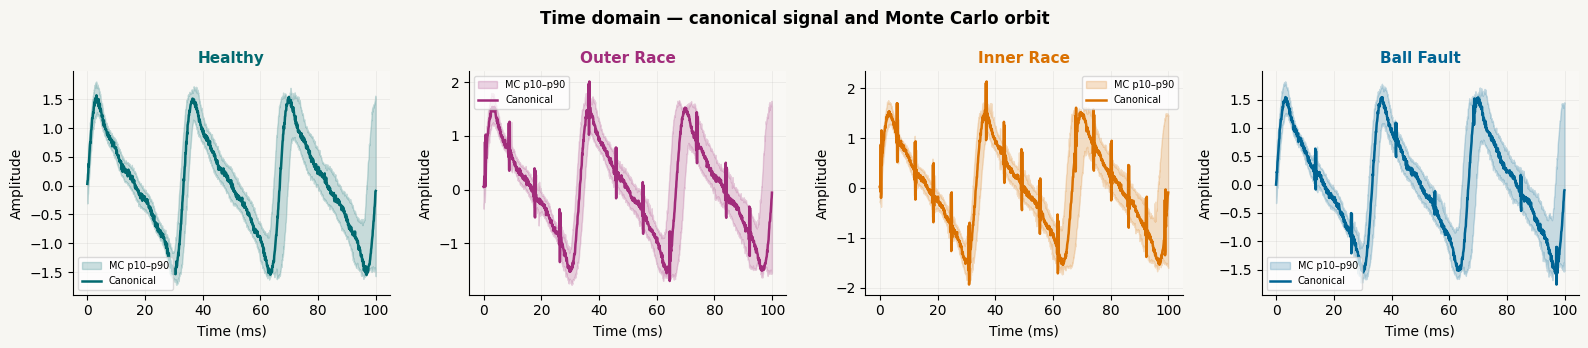
\includegraphics[width=0.92\textwidth]{figures/sim_reconstruction_examples.png}
\caption{
Controlled bearing signal instantiation.
The nominal signal and the non-nominal fault regimes are generated from distinct physical templates, while nuisance transformations modify the observed waveform without changing the intended latent regime.
}
\label{fig:mc_generation}
\end{figure}


%------------------------------------------------------------
\subsection{Representation Operator}
%------------------------------------------------------------

Let
\[
E:\X\rightarrow\Z
\]
be an encoder and
\[
D:\Z\rightarrow\X
\]
a decoder.
In the present implementation, \(E\) and \(D\) are realised by a Conv1D autoencoder trained exclusively on nominal synthetic windows. Autoencoders have long been used as nonlinear representation learners~\cite{hinton2006} and as reconstruction-based anomaly detectors~\cite{sakurada2014}.

The learned reconstruction is
\begin{equation}
\hat{x} = D(E(x)).
\label{eq:reconstruction}
\end{equation}

The reconstruction residual is
\begin{equation}
\residual(x) = \frac{1}{n}\|x-\hat{x}\|_2^2.
\label{eq:residual}
\end{equation}

The residual is interpreted as a computable proxy for distance to the learned nominal structure:
\begin{equation}
\residual(x) \approx d([x],\Mnominal).
\label{eq:distance_proxy}
\end{equation}

This interpretation is important.
The contribution is not the use of mean-squared error as such.
The contribution is the use of a residual as an operational test for membership in the nominal quotient manifold.
In this implementation, the residual is a reconstruction error; in another implementation, it could be replaced by a latent likelihood, an energy score, a predictive error, or a physics-informed residual.

The autoencoder used in the controlled experiment is a one-dimensional convolutional reconstruction model operating directly on fixed-length vibration windows.
The encoder applies successive temporal convolution and compression operations to map each window to a finite-dimensional latent representation.
The decoder mirrors this operation through upsampling and convolutional reconstruction layers.
The model is trained only on nominal synthetic windows by minimizing mean-squared reconstruction error.
No non-nominal samples are used during training.

\begin{table}[H]
\centering
\caption{
Computational role of the autoencoder in the controlled experiment.
}
\label{tab:autoencoder_role}
\begin{tabular}{ll}
\toprule
Component & Role \\
\midrule
Input & Fixed-length vibration window \(x \in \X\) \\
Encoder \(E\) & Maps \(x\) to latent representation \(z \in \Z\) \\
Decoder \(D\) & Reconstructs \(\hat{x}=D(E(x))\) \\
Training data & Nominal synthetic windows only \\
Loss & Mean-squared reconstruction error \\
Diagnostic score & Residual \(r(x)=n^{-1}\|x-\hat{x}\|_2^2\) \\
\bottomrule
\end{tabular}
\end{table}

The architectural choice is intentionally not part of the mathematical formulation.
It is used here as a simple self-supervised operator capable of learning a compact reconstruction model for the nominal nuisance orbit.
Other representation operators could replace it without changing the quotient-space formulation.

\begin{figure}[H]
\centering
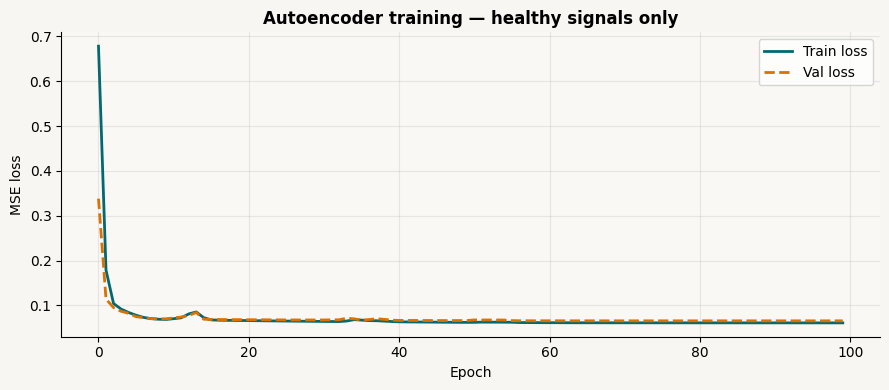
\includegraphics[width=0.88\textwidth]{figures/sim_training_curve.png}
\caption{
Self-supervised learning of a nominal reconstruction operator from synthetic nuisance-orbit samples.
The learned operator is used as one computational approximation of the nominal quotient geometry.
}
\label{fig:training_curve}
\end{figure}

%------------------------------------------------------------
\subsection{Monte Carlo Calibration}
\label{subsec:mc_calibration}
%------------------------------------------------------------

A Monte Carlo reference threshold is estimated from residuals on held-out nominal synthetic samples.
Let
\[
\mcmu = \mathbb{E}_{\mathrm{MC}}[\residual(x)],
\qquad
\mcsigma = \mathrm{Std}_{\mathrm{MC}}[\residual(x)].
\]

More generally, let \(q \in (0,1)\) denote an operational quantile controlling the trade-off between sensitivity and false-alarm tolerance.
A parametric calibration can be written as
\begin{equation}
\tau_{\mathrm{MC}}(q)
=
\mcmu + z_q \mcsigma,
\label{eq:tau_mc_quantile}
\end{equation}
where \(z_q\) is the corresponding standard-normal quantile or an empirically estimated equivalent.
Alternatively, \(\tau_{\mathrm{MC}}(q)\) can be estimated directly as the empirical \(q\)-quantile of the nominal residual distribution.

The value of \(q\) is not part of the mathematical formulation.
It is an operational risk parameter.
Lower values increase sensitivity but may increase false alarms; higher values reduce false alarms but may delay detection of weak or incipient deviations.

In the synthetic experiment reported below, \(q\) is treated as a calibration parameter.
The resulting \(\tau_{\mathrm{MC}}(q)\) defines a reference boundary for the learned nominal structure.

\begin{figure}[H]
\centering
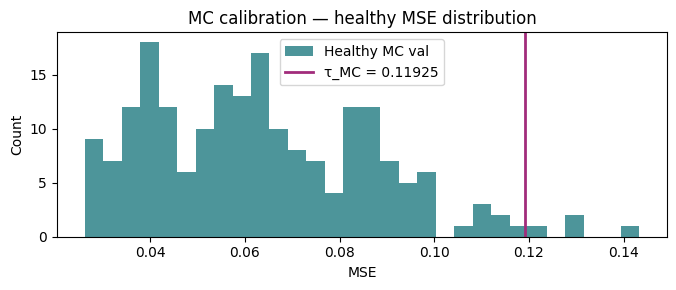
\includegraphics[width=0.88\textwidth]{figures/sim_tau.png}
\caption{
Monte Carlo calibration of the nominal residual distribution.
The threshold defines a synthetic reference boundary for the learned nominal quotient structure.
}
\label{fig:mc_threshold}
\end{figure}

%------------------------------------------------------------
\subsection{Per-Asset Adaptive Threshold}
%------------------------------------------------------------

A global threshold is insufficient when multiple physical assets have different local baselines.
Even if they share the same representation operator, each asset may have a distinct residual scale due to installation, operating conditions, sensor coupling, or local environmental effects.

For each asset \(b\), an adaptive threshold is estimated from a sliding buffer of recent non-anomalous residuals:
\begin{equation}
\tau_t^{(b)}(q)
=
\mu_t^{(b)} + z_q\sigma_t^{(b)}.
\label{eq:adaptive_tau}
\end{equation}

Here \(\mu_t^{(b)}\) and \(\sigma_t^{(b)}\) are computed locally for asset \(b\).
The scalar \(z_q\) preserves the statistical meaning of the selected operational risk level, while the local mean and standard deviation adapt the threshold to each physical asset.

The anomaly decision is
\begin{equation}
a_t^{(b)}
=
\begin{cases}
1, & \residual(x_t^{(b)}) > \tau_t^{(b)}(q),\\
0, & \residual(x_t^{(b)}) \leq \tau_t^{(b)}(q).
\end{cases}
\label{eq:decision_rule}
\end{equation}

This separates the representation problem from the operational decision problem.
The representation is shared across assets.
The decision boundary is local.
In the bearing experiment, each physical asset \(b\) corresponds to one simulated bearing; in the general formulation, \(b\) may represent any monitored component, subsystem, or sensorized physical unit.

%-----------------------------------------------------------------------------
\section{Synthetic Validation}
%-----------------------------------------------------------------------------

The objective of the synthetic experiment is not to prove the quotient-space formulation.
Proposition~\ref{prop:quotient_diagnosis} is a structural statement about diagnostic geometry under nuisance-preserving transformations.
The experiment addresses a different question: whether one computational approximation can recover a residual that behaves as a useful proxy for distance to the nominal quotient manifold.

The validation has four purposes:

\begin{enumerate}[label=(\roman*)]
    \item verify that the simulated nuisance orbits exhibit saturation toward bounded functional regimes;
    \item verify that a representation trained only on nominal trajectories produces low residuals on nominal observations;
    \item verify that non-nominal regimes produce systematically larger residuals without being used during training;
    \item verify that local adaptive thresholds convert the residual into stable per-asset membership decisions.
\end{enumerate}

The controlled instantiation uses four simultaneous synthetic bearings.
Each bearing is treated as one physical asset:

\begin{itemize}
    \item Asset A: nominal throughout the sequence;
    \item Asset B: outer-race fault onset;
    \item Asset C: inner-race fault onset;
    \item Asset D: ball-fault onset.
\end{itemize}

The representation operator is trained only on nominal synthetic data.
Non-nominal regimes are used only for evaluation.
The calibration quantile \(q\) is treated as an operational risk parameter, as defined in Equation~\eqref{eq:tau_mc_quantile}.
In the experiment reported here, adaptive thresholds are estimated using a sliding window of 200 samples unless otherwise stated.

%-----------------------------------------------------------------------------
\subsection{Blueprint Saturation}
%-----------------------------------------------------------------------------

The term \emph{blueprint saturation} follows the companion technical report on self-supervision, manifold saturation, and emergent operational classes~\cite{disanti2026}. 
In that context, a blueprint denotes the finite sampled approximation of a functional regime, and saturation refers to the stabilization of geometric descriptors as the number of samples increases. Here we reuse the same diagnostic to test whether Monte Carlo samples from each simulated regime approach a bounded functional structure.

Before evaluating anomaly decisions, we first examine whether the simulated regimes exhibit blueprint saturation in the sense of~\cite{disanti2026}.
Figure~\ref{fig:blueprint_saturation} reports a blueprint-saturation diagnostic: the p98 manifold radius in a two-dimensional PCA projection as a function of the number of Monte Carlo samples.

The purpose of this diagnostic is not to define the quotient space through PCA.
Rather, it tests whether the sampled nuisance orbits approach bounded functional structures as the number of samples increases.
The stabilization of the p98 radius across regimes suggests that the simulated observations are not merely isolated waveform examples, but samples from compact functional regimes.
This is consistent with the quotient-space interpretation: nuisance variability expands the raw observation cloud, but the orbit generated by a fixed latent regime remains geometrically bounded.

\begin{figure}[H]
\centering
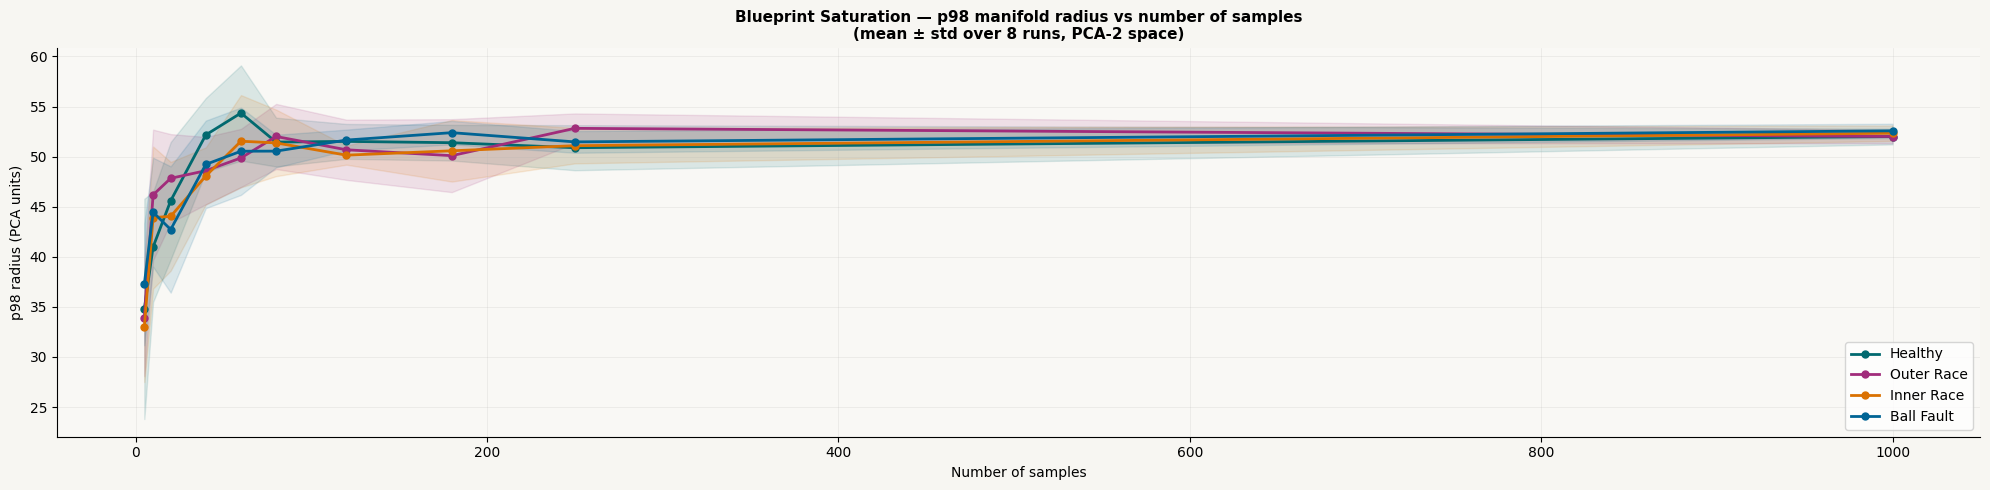
\includegraphics[width=0.88\textwidth]{figures/sim_blueprint_saturation.png}
\caption{
Blueprint saturation of the simulated functional regimes, following the manifold-saturation diagnostic introduced in~\cite{disanti2026}.
For each regime, the p98 manifold radius is estimated in a two-dimensional PCA projection as the number of Monte Carlo samples increases.
The stabilization of the radius indicates that the sampled nuisance orbit approaches a bounded functional structure.
This supports the interpretation that the simulator generates compact quotient-space regimes rather than isolated waveform examples.
}
\label{fig:blueprint_saturation}
\end{figure}

%-----------------------------------------------------------------------------
\subsection{Residual Separation}
%-----------------------------------------------------------------------------

Figure~\ref{fig:mse_distributions} shows the residual distributions obtained after training the representation operator on nominal trajectories only.
The important point is not that the residual is mean-squared error in this implementation.
The important point is that the residual behaves as a proxy for membership in the learned nominal structure.
Nominal observations concentrate at low residual values, while non-nominal regimes shift to higher residual regions.

\begin{figure}[H]
\centering
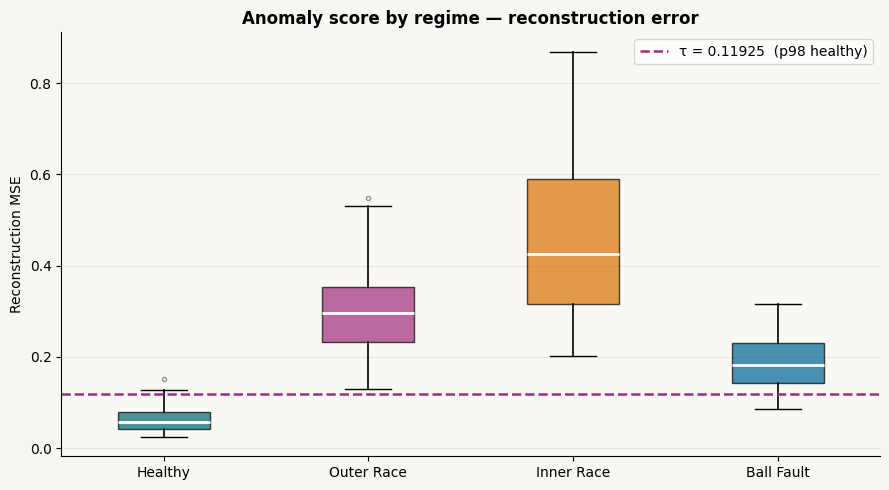
\includegraphics[width=0.88\textwidth]{figures/sim_mse_distributions.png}
\caption{
Residual distributions produced by the learned representation operator.
The operator is trained only on nominal trajectories.
The separation between nominal and non-nominal regimes indicates that the learned residual is diagnostically meaningful as a proxy for distance to the nominal quotient manifold.
}
\label{fig:mse_distributions}
\end{figure}

%-----------------------------------------------------------------------------
\subsection{Adaptive Window Robustness}
%-----------------------------------------------------------------------------

The adaptive boundary depends on a sliding window of recent residuals.
To test whether the result is sensitive to this choice, we evaluate false-alarm and detection rates across several window sizes.
Figure~\ref{fig:window_sensitivity} shows that the detection rate remains high while the false-alarm rate remains low across a broad range of window sizes.
Thus, the adaptive decision rule is not an artefact of a single hand-tuned window length.

\begin{figure}[H]
\centering
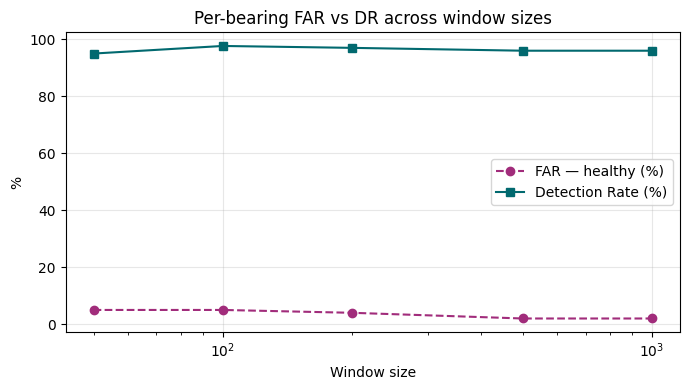
\includegraphics[width=0.78\textwidth]{figures/sim_window_sensitivity.png}
\caption{
Sensitivity of the adaptive decision rule to the sliding-window size.
The detection rate remains high across a wide range of window sizes, while the false-alarm rate remains low.
This indicates that the per-asset adaptive boundary is not an artefact of a single window choice.
}
\label{fig:window_sensitivity}
\end{figure}

%-----------------------------------------------------------------------------
\subsection{Per-Asset Detection Results}
%-----------------------------------------------------------------------------

Table~\ref{tab:synthetic_results} reports the resulting membership decisions after applying the adaptive threshold.
FAR denotes the false-alarm rate during nominal operation.
DR denotes the detection rate after non-nominal onset.

\begin{table}[H]
\centering
\caption{
Synthetic per-asset detection metrics.
The representation operator is shared across all assets, while the adaptive decision boundary is estimated locally for each asset.
}
\label{tab:synthetic_results}
\begin{tabular}{llcc}
\toprule
Asset & Scenario & FAR during nominal period & DR after onset \\
\midrule
A & Nominal throughout       & 1.5\% & N/A \\
B & Outer-race fault onset   & 2.0\% & 100\% \\
C & Inner-race fault onset   & 2.0\% & 100\% \\
D & Ball-fault onset         & 2.0\% & 86\% \\
\bottomrule
\end{tabular}
\end{table}

The results show that the learned residual remains stable for the asset that remains nominal and increases after non-nominal onset for the remaining assets.
The outer-race and inner-race regimes are detected completely in the evaluation interval.
The ball-fault regime is detected less strongly, with an 86\% detection rate, which is consistent with a weaker or less separable deviation from the learned nominal structure.

These numbers should be interpreted as preliminary evidence of operational feasibility, not as a claim of benchmark-level performance.
The scientific claim of this note is the quotient-space inverse formulation.
The synthetic experiment demonstrates that one computational realization of that formulation can produce useful membership decisions.

%-----------------------------------------------------------------------------
\section{Interpretation}
%-----------------------------------------------------------------------------

The experiment supports four claims.

First, the simulated regimes exhibit blueprint saturation in the sense of the companion report~\cite{disanti2026}: as the number of Monte Carlo samples increases, the p98 radius stabilizes, suggesting that the nuisance orbits approach bounded functional structures. This supports the use of the synthetic emulator as a controlled setting for studying quotient-space recovery.

Second, a representation trained only on nominal nuisance-orbit samples can produce residuals that distinguish nominal and non-nominal regimes. This is consistent with the interpretation of the residual as a proxy for distance to the nominal quotient manifold.

Third, the adaptive boundary should be estimated locally for each physical asset. A shared representation can be global, but the decision boundary must account for local residual baselines. This reflects the distinction between learning a common quotient geometry and estimating an asset-local operational boundary.

Fourth, non-nominal regimes need not be learned as semantic labels. In the controlled bearing experiment, outer-race, inner-race, and ball-fault regimes are detected by departure from the nominal structure. This is the inverse-problem view: first recover membership in the nominal functional structure; assign semantics later.

%-----------------------------------------------------------------------------
\section{Discussion}
%-----------------------------------------------------------------------------

The proposed formulation differs from standard supervised fault classification in three ways.

\paragraph{Diagnosis precedes classification.}
The primary decision is whether an observation belongs to the nominal quotient manifold.
Classification of the type of non-nominal condition is a subsequent semantic step.

\paragraph{The representation is geometric.}
The goal is not to memorize labels, but to collapse nuisance orbits while preserving latent physical-state information.
This is why the quotient space is the natural object.

\paragraph{The threshold is asset-local.}
A physical asset may have a local residual baseline even when the representation operator is shared.
Per-asset adaptive thresholding estimates this local boundary without retraining the representation.

This work also clarifies the relationship between quotient spaces and functional manifolds.
The quotient-space formulation provides the geometric mechanism through which functional manifolds emerge.
They are connected regions of the quotient space after nuisance directions have been collapsed.
This gives a mathematical origin to the compact structures observed in self-supervised diagnostic representations.

%-----------------------------------------------------------------------------
\section{Limitations}
%-----------------------------------------------------------------------------

This work should not be read as a complete industrial validation.

The current experiment is synthetic.
It demonstrates the feasibility of one computational approximation under controlled conditions, but it does not establish robustness under field conditions.

The synthetic emulator is designed to test the geometry of the proposed formulation under controlled ground-truth conditions; it is not intended to reproduce the full mechanical, tribological, or environmental complexity of field bearing data.

The nuisance transformation family is approximate.
In real machines, nuisance effects may not form an exact mathematical group.
Nevertheless, the quotient-space formulation remains useful as an organizing principle when transformations approximately preserve the physical state.

The autoencoder is only one possible approximation.
Future work should compare reconstruction-based residuals with alternative representation operators and distance functions.

Finally, fault classification is not fully addressed here.
The present work focuses on anomaly detection as failure of membership in the nominal quotient manifold.
Fault classification can be formulated as identifying the destination manifold after departure from the nominal structure.

%-----------------------------------------------------------------------------
\section{Conclusion}
%-----------------------------------------------------------------------------

This work establishes a mathematical formulation of diagnostic monitoring as inverse recovery over quotient-space geometry.
The formulation begins with the physical observation model, identifies nuisance transformations that preserve the latent physical state, and shows that diagnosis naturally factors through the quotient space induced by those transformations.

The proposed learning architecture constitutes one practical approximation of that formulation.
Monte Carlo simulation samples the nominal nuisance orbit, a self-supervised representation operator approximates the nominal quotient geometry, and a per-asset adaptive threshold estimates the local decision boundary.
Synthetic experiments provide preliminary empirical evidence that quotient-space recovery is feasible under controlled operating conditions.

The main contribution is therefore not a particular autoencoder architecture or a bearing-specific detector.
The main contribution is the geometric formulation:
anomaly detection can be posed as a membership problem on quotient-space functional manifolds induced by nuisance-invariant observations.

Future work will investigate field validation, alternative representation operators, fault-manifold classification after anomaly detection, and transfer to industrial rotating machinery datasets.

%-----------------------------------------------------------------------------
\section*{Accompanying Source Material}
%-----------------------------------------------------------------------------

The synthetic bearing emulator, Monte Carlo generation scripts, Conv1D autoencoder training notebook, adaptive-threshold calibration code, and figure-generation scripts are deposited as accompanying source material for this work.
The source material is provided to make the controlled validation reproducible and to distinguish the general quotient-space formulation from the particular computational approximation used in the experiment.

%-----------------------------------------------------------------------------
\begin{thebibliography}{99}

\bibitem{hadamard}
J. Hadamard.
\newblock \emph{Lectures on Cauchy's Problem in Linear Partial Differential Equations}.
\newblock Yale University Press, 1923.

\bibitem{tikhonov}
A. N. Tikhonov and V. Y. Arsenin.
\newblock \emph{Solutions of Ill-Posed Problems}.
\newblock Winston, 1977.

\bibitem{chandola2009}
V. Chandola, A. Banerjee, and V. Kumar.
\newblock Anomaly detection: A survey.
\newblock \emph{ACM Computing Surveys}, 41(3), Article 15, 2009.

\bibitem{scholkopf1999}
B. Sch\"olkopf, R. C. Williamson, A. J. Smola, J. Shawe-Taylor, and J. C. Platt.
\newblock Support vector method for novelty detection.
\newblock In \emph{Advances in Neural Information Processing Systems}, 1999.

\bibitem{bishop1994}
C. M. Bishop.
\newblock Novelty detection and neural network validation.
\newblock \emph{IEE Proceedings --- Vision, Image and Signal Processing}, 141(4), 1994.

\bibitem{kohonen}
T. Kohonen.
\newblock Self-organized formation of topologically correct feature maps.
\newblock \emph{Biological Cybernetics}, 43, 59--69, 1982.

\bibitem{hinton2006}
G. E. Hinton and R. R. Salakhutdinov.
\newblock Reducing the dimensionality of data with neural networks.
\newblock \emph{Science}, 313(5786), 504--507, 2006.

\bibitem{sakurada2014}
M. Sakurada and T. Yairi.
\newblock Anomaly detection using autoencoders with nonlinear dimensionality reduction.
\newblock In \emph{Proceedings of the 2nd Workshop on Machine Learning for Sensory Data Analysis}, 2014.

\bibitem{bronstein2021}
M. M. Bronstein, J. Bruna, T. Cohen, and P. Veli\v{c}kovi\'c.
\newblock Geometric deep learning: Grids, groups, graphs, geodesics, and gauges.
\newblock \emph{arXiv:2104.13478}, 2021.

\bibitem{jardine2006}
A. K. S. Jardine, D. Lin, and D. Banjevic.
\newblock A review on machinery diagnostics and prognostics implementing condition-based maintenance.
\newblock \emph{Mechanical Systems and Signal Processing}, 20(7), 1483--1510, 2006.

\bibitem{randall2011}
R. B. Randall and J. Antoni.
\newblock Rolling element bearing diagnostics---A tutorial.
\newblock \emph{Mechanical Systems and Signal Processing}, 25(2), 485--520, 2011.

\bibitem{cwru_benchmark}
W. A. Smith and R. B. Randall. 
\newblock Rolling element bearing diagnostics using the Case Western Reserve University data: A benchmark study.
\newblock \emph{Mechanical Systems and Signal Processing}, 64--65, 100--131, 2015.

\bibitem{zhao2019}
R. Zhao, R. Yan, Z. Chen, K. Mao, P. Wang, and R. X. Gao.
\newblock Deep learning and its applications to machine health monitoring: A survey.
\newblock \emph{Mechanical Systems and Signal Processing}, 115, 213--237, 2019.

\bibitem{lei2013}
Y. Lei, J. Lin, Z. He, and M. J. Zuo.
\newblock A review on empirical mode decomposition in fault diagnosis of rotating machinery.
\newblock \emph{Mechanical Systems and Signal Processing}, 35(1--2), 108--126, 2013.

\bibitem{disanti2026}
E. Di Santi.
\newblock \emph{Self-Supervision, Manifold Saturation, and Emergent Operational Classes: Learning from Scarce Observations as Inverse Recovery of Compact Functional Structure}.
\newblock Technical report, University of Colorado Boulder, 2026.

\end{thebibliography}

\end{document}
